\documentclass[a4paper, 20pt]{article}
\usepackage[english]{babel}
\usepackage{amsmath}
\usepackage{graphicx}
\usepackage{subcaption}
\usepackage{placeins}
\usepackage[T1]{fontenc}
\usepackage[utf8]{inputenc}
\usepackage{floatrow}

\author{Maarten de Jonge \\
    Inge Becht}
\date{\today}
\title{Assignment 3\\ 
Probabilistic Pose Estimation based on Topological Map}

\begin{document}
\maketitle

In this assignment it was attempted to create a topological map of 3 different
rooms using an omni camera (as was used in the previous assignment). Two
different ways of topological mapping were attempted; using wall extraction
and by using colored blobs. In the first case landmarks were determined by
finding sequences of wall parts and corridors, and in the second case the
orientation of the colored blobs were used to determine the position of the
legorobot.
These sequences, called fingerprints, could in theory be used to distinguish between
the three different rooms, as long as the fingerprints differ enough.

\section{The dataset} 
The dataset consists of multiple pictures of every room, each with a different
orientation of the robot within the room. This will create different possible
fingerprints for both the wall based topological mapping as well as the blob
based mapping. By rotating the sequences of these fingerprints it should be
clear that two fingerprints are so much alike they refer to the same room, while
reducing the noise in the fingerprints. Figure \ref{fig:exdata} shows one of the
images from the dataset.

\begin{figure}[!ht]
\centering
  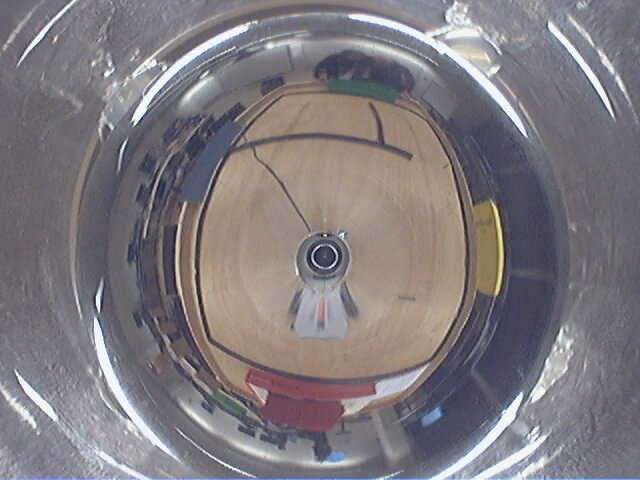
\includegraphics[width=0.5\textwidth]{data_set/2012-11-26-121531.jpg}
  \label{fig:exdata}
  \caption{A picture from the dataset. Represented is room 3.} 
\end{figure}

\section{Using wall extraction for localisation}
In the previous assignment we were able to succesfully find data points that
represented walls of our lego construction. This same method is now used in this
assignment (see figure \ref{fig:wallpoints}). The next step towards creating the 
final fingerprints is to first  map these points to line segments, as seen in
\ref{fig:wall_lines}

\begin{figure}[!ht]
\centering
\begin{floatrow}
    \ffigbox[\FBwidth]{\caption{A picture of all extracted wallpoints from room
    3}\label{fig:wallpoints}}{
    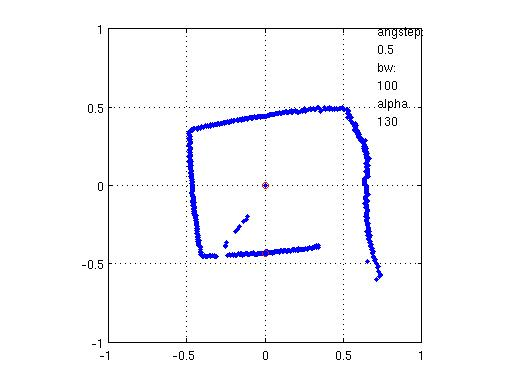
\includegraphics[width=0.5\textwidth]{Results/points_room3.jpg}}
  
  \ffigbox[\FBwidth]{\caption{A picture of all extracted lines from room 3}
  \label{fig:wall_lines}}{
  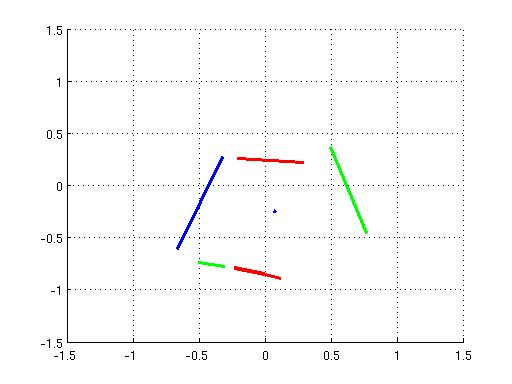
\includegraphics[width=0.5\textwidth]{Results/Lines_room3.jpg}}
\end{floatrow}
\end{figure}

With these line segments we are now able to create a fingerprint. Depending on
the size of the \texttt{angstep} (the same variable from the previous exercise)
. The \texttt{angstep} determines the angle between every laser step, and in
this case also the step for each sequence in the fingerprint.

\section{Using color blobs for localisation}
Colors need to be detected by determining the right threshold in HSL values for
all four of the colors. Because all blobs are not exactly one color bus fall in
a range of hues (due to shadow forming and light direction) all colors have a
maximum and minimum hue that is used.  
The original image gets thresholded on these values and
after that the biggest blob is extracted by using the matlab function
\texttt{bwlabel}.


\begin{figure}[!ht]
\centering
\begin{floatrow}
    \ffigbox[\FBwidth]{\caption{\texttt{imunwrap.m}Image after initial
    thresholding}\label{fig:angstep0.05}}{
    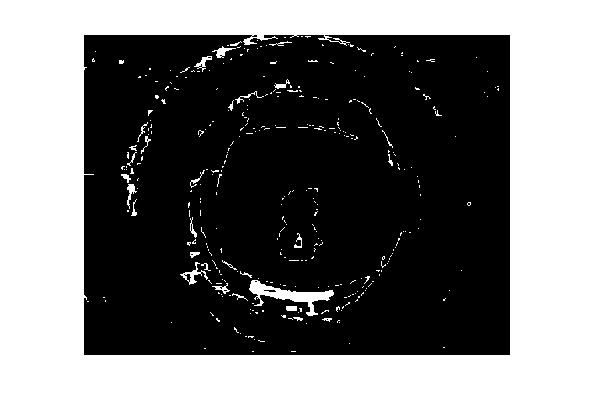
\includegraphics[width=0.5\textwidth]{Results/red_thresh_room3.jpg}}
  
  \ffigbox[\FBwidth]{\caption{\texttt{imunwrap.m} Image with final blob detected}
  \label{fig:angstep5}}{
  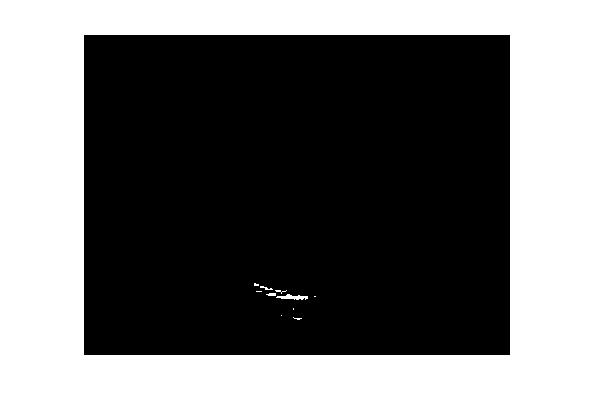
\includegraphics[width=0.5\textwidth]{Results/red_threshlabel_room3.jpg}}
\end{floatrow}
\end{figure}

The provided script only works with two colors at one time to create the
fingerprint, so we devide the colors used for every room. This makes the problem
of identifying a room
a lot more straightforward, as now one of the two colors can always be chosen
uniquely. This is not all that unrealistic as color blobs could be the color of
walls in the room or other keyfeatures. The script \texttt{ComputePatStringBlobs.m} gives the option to return
the fingerprint with only a value 3 for every blob without discriminating
between
the colors.
For room 3 we use colors red and yellow. For room 2 we use colors green and
yellow and for room 1 we use colors blue and green. 


\section{Comparing fingerprints using Levenshtein distance}
Now that ways have been determined to establish the fingerprints, these
fingerprints now need to be compared some way or the other. Because these
fingerprints are nothing more than a row of characters that determine if
given some radius step there is a, the Levenshtein distance can be used for
this. The Levenshtein distance is a way to measure the \texttt{distance}
between two sequences by determining how many deletions, replacements and
insertions have to be made to end up with two the same sequences. In our use of
the fingerprints only the replacement operation will be important as we use one
and the same \texttt{angstep} for every fingerprint extraction.

If we want to measure the difference between two fingerprints we first need to
rotate both strings so that we know for sure the orientation of the robot plays
no part in the final distance calculation (for example if we want to compare a
fingerprint of room 1 with another for room 1, it may not look the same in case
the robot looks the other direction and thus the sequence is the same but each
element is at another place). The way we chose to neglect this rotiation is by
putting the first element of one of the fingerprints after the last one until we
end up with this character at the beginning again, at every step calculating how
big the Levenshtein difference is. When it is at a minimum we know that we have
compensated for the rotiation of the robot.

In \texttt{find\_distance.m} the strings are rotated and returned the absolute minimal
Levenshtein distance (using the code provided in \texttt{LevenshteinDistance.m}) that could be found.

Now that the fingerprints have been made rotation invariant, we need to make a
dataset for each room with same orientations, which can be done while running
\texttt{GetLinePattern.m} and \texttt{GetBlobPattern.m} respectively. These
files create a \texttt{.mat} file with encoded fingerprints.



\section{Experiments and Results}
A script was written to match a fingerprint against each fingerprint in the
labeled set of data to find the most likely location belonging to that
fingerprint.

With 3 different locations and 11 different tested fingerprints, there is a
success-rate of 63\%, which is okay. The set of fingerprints used for testing
are the same as used for the labeled data, so it isn't the most scientifically
valid test. It does however demonstrate that the algorithm works, and
performs significantly better than random guessing would.

\end{document}
